\documentclass[a4paper,10pt]{article}

\usepackage[latin1]{inputenc}
\usepackage[spanish]{babel}
\usepackage{fontenc}
\usepackage{graphicx}
\usepackage{verbatim}
\author{Santiago Videla}
\title{vac-o\\ Documento de Dise\~no}
\pagestyle{headings}

\begin{document}
\maketitle
\newpage
\tableofcontents
\newpage
\section{Introducci\'on}
  \subsection{Prop\'osito}
  El prop\'osito de este documento es presentar el dise\~no de vac-o. La
tecnica adoptada para realizar el analisis y descripci\'on del mismo se
denomina ``Dise\~no dirigido por responsabilidades'' (Responsability-driven
design) descripto en un \textit{paper} de Rebecca Wirfs-Brock y Brian
Wilkerson, ``Object-Oriented Design: A Responsibility-Driven Approach''.

  \subsection{Descripci\'on general del documento}
  En la secci\'on~\ref{hld} se presenta el dise\~no de alto nivel del sistema,
sus interfaces y paquetes principales.

  En la secci\'on~\ref{lld} se presenta el dise\~no de bajo nivel del sistema,
las clases concretas y sus relaciones para cada paquete.

  \section{Dise\~no de alto nivel}
\subsection{Interfaces - Responsabilidades - Colaboradores}
\begin{figure}
  \centering
  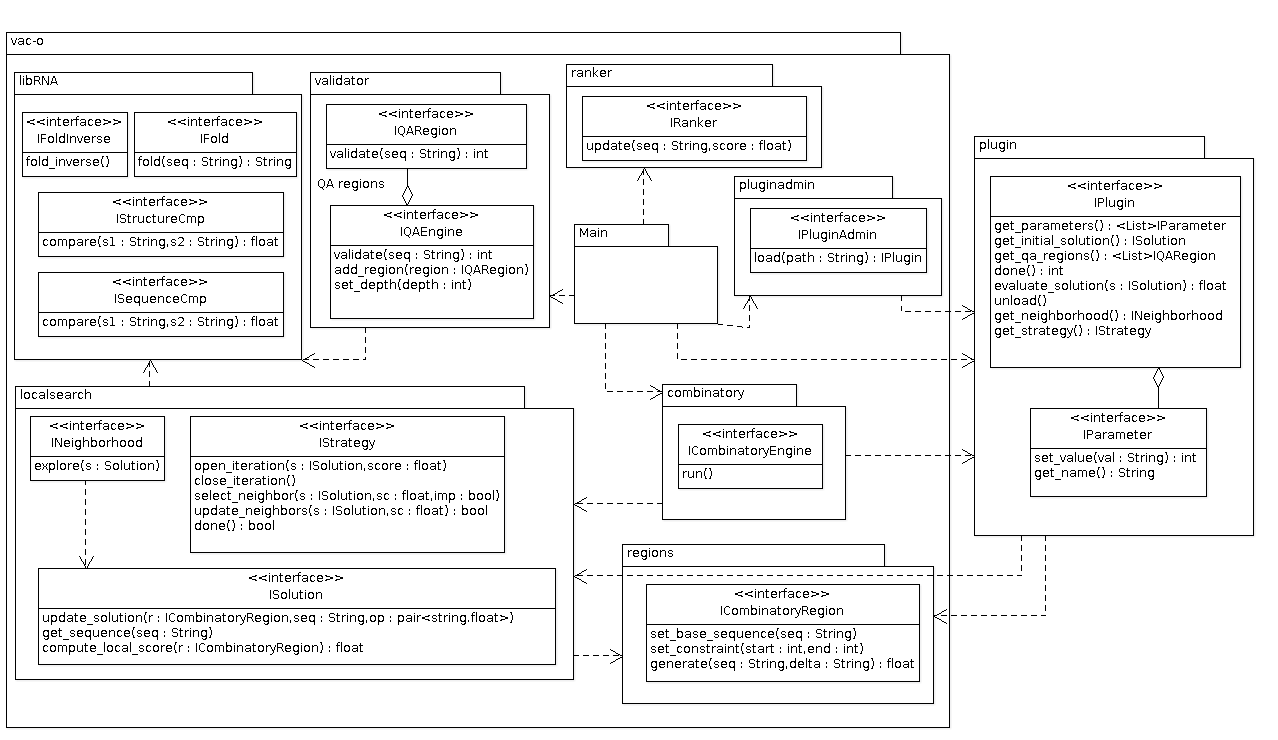
\includegraphics[scale=0.5, angle=90]{hld.png}  
  \caption{UML - Interfaces}
  \label{uml:1}
\end{figure}

  \subsubsection{IPluginAdmin}
    \paragraph{Responsabilidad:} Administrar las extensiones del sistema
(archivos \textit{.so}).    
      \begin{enumerate}
       \item Cargar extensi\'on.       
      \end{enumerate}    

  \subsubsection{IPlugin}
    \paragraph{Responsabilidad:} Brindar la informaci\'on y servicios
particulares para una vacuna determinada.    
      \begin{enumerate}
       \item Proveer la lista de par\'ametros requeridos por la extensi\'on.
       \item Proveer la secuencia de ARN que se encuentra en la cepa vacunal.
       \item Proveer las regiones combinatorias que se deben usar para buscar
mejoras a la vacuna.
       \item Proveer el umbral que se debe usar para determinar la bondad de las
secuencias obtenidas de las regi\'ones combinatorias.
       \item Proveer las regiones de validaci\'on que se deben usar para
realizar el control de calidad.
       \item Determinar si se continua buscando secuencias o no.
       \item Evaluar las secuencias candidatas.
       \item Descargar la extensi\'on.
      \end{enumerate}
    \paragraph{Colaboradores:}
      \begin{enumerate}
       \item \textbf{BioPP:} Calculo de distancias entre secuencias.
       \item \textbf{LibPlugin}: Factories de regiones combinatorias y de
validaci\'on.
      \end{enumerate}

  \subsubsection{ICombinatoryRegion}
    \paragraph{Responsabilidad:} Calcular las secuencias que mantengan
determinadas propiedades de una secuencia original.    
      \begin{enumerate}
       \item Devolver la siguiente secuencia.
       \item Evaluar la bondad de una secuencia.
      \end{enumerate}
    \paragraph{Colaboradores:}
      \begin{enumerate}
       \item \textbf{BioPP:} Calculo de secuencias que mantengan una propiedad
determinada (estructura secundaria, c\'odigo gen\'etico, etc).
      \end{enumerate}

  \subsubsection{ICombinatoryEngine}
    \paragraph{Responsabilidad:} Generar secuencias candidatas a partir de las
variantes generadas de cada regi\'on combinatoria.       
      \begin{enumerate}       
       \item Inicializar las regiones combinatorias.
       \item Devolver la siguiente secuencia candidata.
      \end{enumerate}
    \paragraph{Colaboradores:}
      \begin{enumerate}
       \item \textbf{ICombinatoryRegion:} Consulta la siguiente secuencia de
cada regi\'on combinatoria.
      \end{enumerate}

  \subsubsection{IQAMutator}
    \paragraph{Responsabilidad:} Generar mutaciones de una secuencia
utilizando alg\'un criterio (todas las mutaciones posibles, $N$
mutaciones aleatorias, etc).
      \begin{enumerate}
       \item Devolver la siguiente mutaci\'on.
      \end{enumerate}    

  \subsubsection{IQAValidator}
    \paragraph{Responsabilidad:} Decidir si una secuencia satisface o
mantiene determinadas propiedades.
    \paragraph{Colaboradores:}
      \begin{enumerate}
       \item \textbf{BioPP:} Calculo y comparaci\'on de estructura secundaria o
conteo de nucle\'otidos
      \end{enumerate}

  \subsubsection{IQARegion}
    \paragraph{Responsabilidad:} Realizar el control de calidad para una
regi\'on de validaci\'on.
      \begin{enumerate}
       \item Calcular y validar mutaciones acumuladas de la regi\'on hasta
alcanzar la profundidad deseada.
      \end{enumerate}
    \paragraph{Colaboradores:}
      \begin{enumerate}
       \item \textbf{IQAMutator:} Consulta la siguiente mutaci\'on.
       \item \textbf{IQAValidator:} Consulta si una mutaci\'on determinada es
valida o no.
      \end{enumerate}

  \subsubsection{IQAEngine}
    \paragraph{Responsabilidad:} Realizar el control de calidad para una
secuencia candidata.
      \begin{enumerate}       
       \item Inicializar regiones de validaci\'on.
       \item Determinar si una secuencia candidata aprueba o no el control de
calidad para todas sus regiones de validaci\'on.
      \end{enumerate}
    \paragraph{Colaboradores:}
      \begin{enumerate}
       \item \textbf{IQARegion:} Consulta si la regi\'on de validaci\'on aprueba
o no el control de calidad.
      \end{enumerate}

  \subsubsection{IRanker}
    \paragraph{Responsabilidad:} Mantener un \textit{ranking} de secuencias en
base al puntaje asignado a cada una.       
    \paragraph{Colaboradores:}
      \begin{enumerate}
       \item \textbf{IPlugin:} Consulta el puntaje para una secuencia
determinada.
      \end{enumerate}

\begin{comment}
  \subsection{Interface}
    \paragraph{Responsabilidad:}    
      \begin{enumerate}
       \item 
      \end{enumerate}
    \paragraph{Colaboradores:}
      \begin{enumerate}
       \item 
      \end{enumerate}
\end{comment}

  \section{Dise\~no de bajo nivel}
\label{lld}  
    \begin{figure}
      \centering
      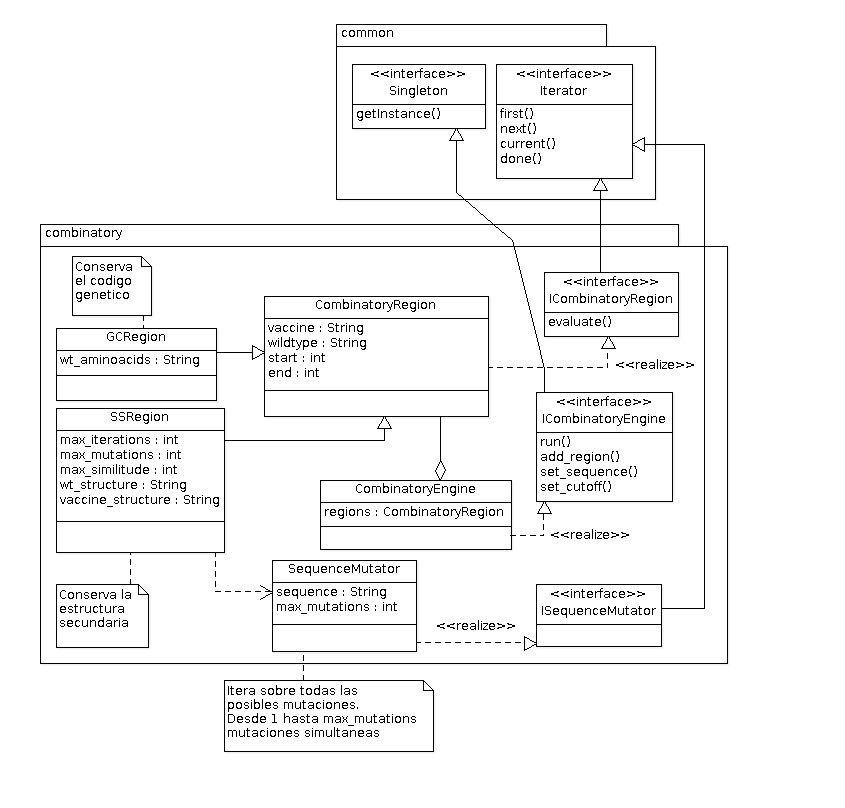
\includegraphics[scale=0.5]{lld-combinatory.png}  
      \caption{UML - Combinatory}
      \label{uml:2}
    \end{figure}

    \begin{figure}
      \centering
      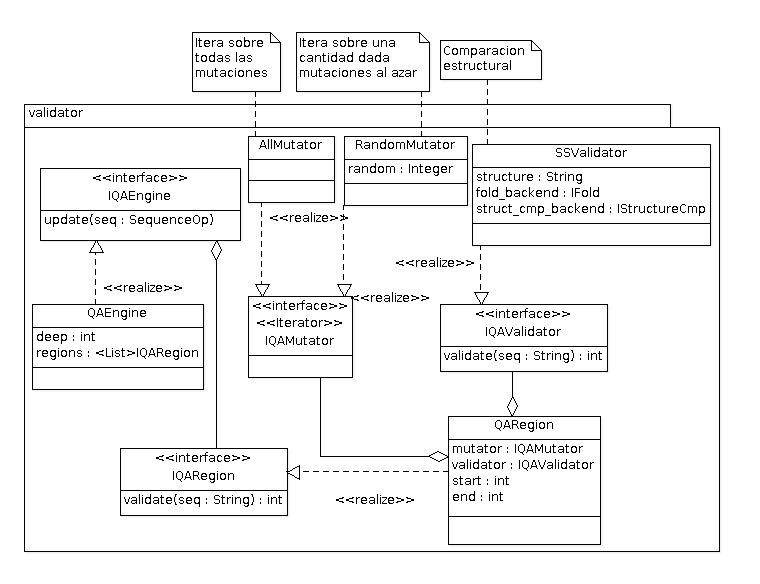
\includegraphics[scale=0.5]{lld-validator.png}  
      \caption{UML - Validator}
      \label{uml:3}
    \end{figure}

\end{document}
